\documentclass[preprint,12pt]{elsarticle}
\usepackage[UTF8,scheme=plain,fontset=fandol]{ctex}
\usepackage{amsmath,amssymb,bm}
\usepackage{booktabs,multirow,threeparttable}
\usepackage{graphicx,subcaption}
\usepackage{siunitx}
\usepackage{xcolor,hyperref,lineno,enumitem}
\graphicspath{{../figures/}}
\hypersetup{colorlinks=true,linkcolor=blue!50!black,citecolor=blue!50!black,urlcolor=blue!60!black}
\emergencystretch=2em
\journal{Transportation Research Part C}
\renewcommand{\figurename}{图}
\renewcommand{\tablename}{表}

\begin{document}
\begin{frontmatter}

\title{面向全生命周期成本与油电混行能耗的高速公路三维线形数据驱动协同优化}

\author[aff1]{匿名作者}
\affiliation[aff1]{organization={双盲审稿匿名单位},city={匿名},country={中国}}

\begin{abstract}
高速公路线形设计同时耦合平面几何、纵断面、地形、桥隧结构、城市建设强度以及长期车辆运行。现有优化模型常对其中若干关系作固定化处理，导致所得方案虽具有较低目标值，却可能在空间、结构或工程经济意义上失真。本文构建面向平纵协同的双目标优化框架，将准天然数字高程模型（DEM）、OpenStreetMap（OSM）道路/铁路/水系与建筑密度分区，以及14,018个实测GNSS轨迹点融合至同一数字走廊。决策向量由50阶低频平面正弦模态和225个纵断面变量组成；全生命周期成本包含占地、基本工程、桥隧、土方和养护，能耗目标将30年油电混合车流的燃油与电耗货币化。候选线形与OSM障碍物相交时内生触发跨越桥，高程连通山体触发生态隧道，高密度建成区核心作为硬禁行区。求解方法采用改进水母搜索算法（IJS），集成独立Tent混沌初始化、按搜索域缩放的L\'evy飞行和差分进化（DE）精修；熵权仅用于可行非支配解的折中决策，不能抵消规范违约。

以广州北环高速浔峰洲—黄村段（22.46 km）为例。在当前“端点高程锚定、走廊带半宽500 m、建筑密度约束开启”的设置下，折中方案将全生命周期成本由26.4061亿元降至24.2078亿元（$-8.33\%$），将货币化车流能耗由13.9460亿元降至13.5278亿元（$-3.00\%$）；最小平曲线半径为421 m，硬约束罚值为0，Tier-2禁行区穿越长度为0，Tier-1穿越长度由约2.00 km降至1.59 km。前一版同口径控制实验表明，先平面后纵断面的两阶段法虽然得到更低表观目标，但最小半径仅397 m，不可行；联合协同方案则满足400 m限值。30次独立消融中，IJS相对原始JS的平均标量目标改善25.45\%，其中DE贡献占主导。六个联合问题规模（95--500维）下，IJS均优于JS、NSGA-II、GA、PSO和GWO，配对Wilcoxon检验均小于$8.8\times10^{-4}$。237个重优化敏感性点全部可行。结果说明，DEM/OSM工程约束与平纵协同不仅提高数值优化质量，也改变了最优解的物理含义和可实施性。
\end{abstract}

\begin{keyword}
高速公路线形优化 \sep 数字高程模型 \sep OpenStreetMap \sep 改进水母搜索算法 \sep 全生命周期成本 \sep 油电混行能耗 \sep 平纵协同
\end{keyword}
\end{frontmatter}

\linenumbers

\section{引言}

高速公路线形一旦在前期确定，将长期影响建设投资、桥隧比例、土石方调配、养护暴露和车辆运行。一条线位的微小横移会改变其所穿越的地面高程、障碍物和建筑区；平面路径缩短可能造成纵断面恶化；绕避山体可能进入高密度建成区；降低土方可能需要增设桥梁；未经端点控制的纵断面还可能利用“起高终低”获得虚假节能。因此，线形优化的核心不是单独拟合一条曲线，而是在空间数据、工程规范和竞争目标共同作用下寻找可实施的三维方案。

早期研究已证明平面与纵断面同步优化的必要性\cite{chew1989,jong2003}。此后，研究者发展了走廊带模型、混合整数方法、环境目标和偏好驱动的多目标搜索\cite{kang2012,mondal2015,hirpa2016,vazquez2018,akhmet2022}；近年又引入BIM、GIS、深度强化学习和采样式路径规划\cite{han2023,he2023,alhadad2024,pu2024}。然而，现有综述仍指出算法模型与真实工程异构约束之间存在明显鸿沟\cite{songreview2023}。

本文针对三类问题展开改进。第一，单一中线高程或理想化地价栅格不能使平面横移真正改变地形，从模型结构上削弱平纵协同。第二，固定桥隧长度和不连续惩罚会给优化器留下“利用计价规则”的空间。第三，高维非线性搜索容易把局部曲率、坡差等违约平均掉，产生目标低而不可行的解。

本文以林坤锐学位论文\cite{lin2025}的全生命周期成本—能耗数学模型为基底，将其以NSGA-II和单中线数据为主的实现扩展为当前数据驱动实验。主要贡献如下：

\begin{enumerate}[leftmargin=*,label=(\arabic*)]
\item 建立GNSS、准天然DEM、OSM交通/水系和建筑密度三级区共同驱动的数字走廊；
\item 建立桥梁交叉触发、生态隧道、土方—结构替代以及接线端点高程内生于三维几何的工程化全生命周期模型；
\item 构建50个平面模态与225个纵断面变量组成的275维平纵协同参数化，并实现成本—油电混行能耗双目标决策；
\item 提出经数值修正的IJS，将独立Tent初始化、L\'evy探索与DE精修结合；
\item 通过方案对比、组件消融、六规模算法对比和237点重优化敏感性形成完整证据链。
\end{enumerate}

图\ref{fig:overview_zh}展示从数据到可行线形的完整流程。图中每个模块均对应仓库中的可复核数据、模型或结果文件。

\begin{figure*}[t]
\centering
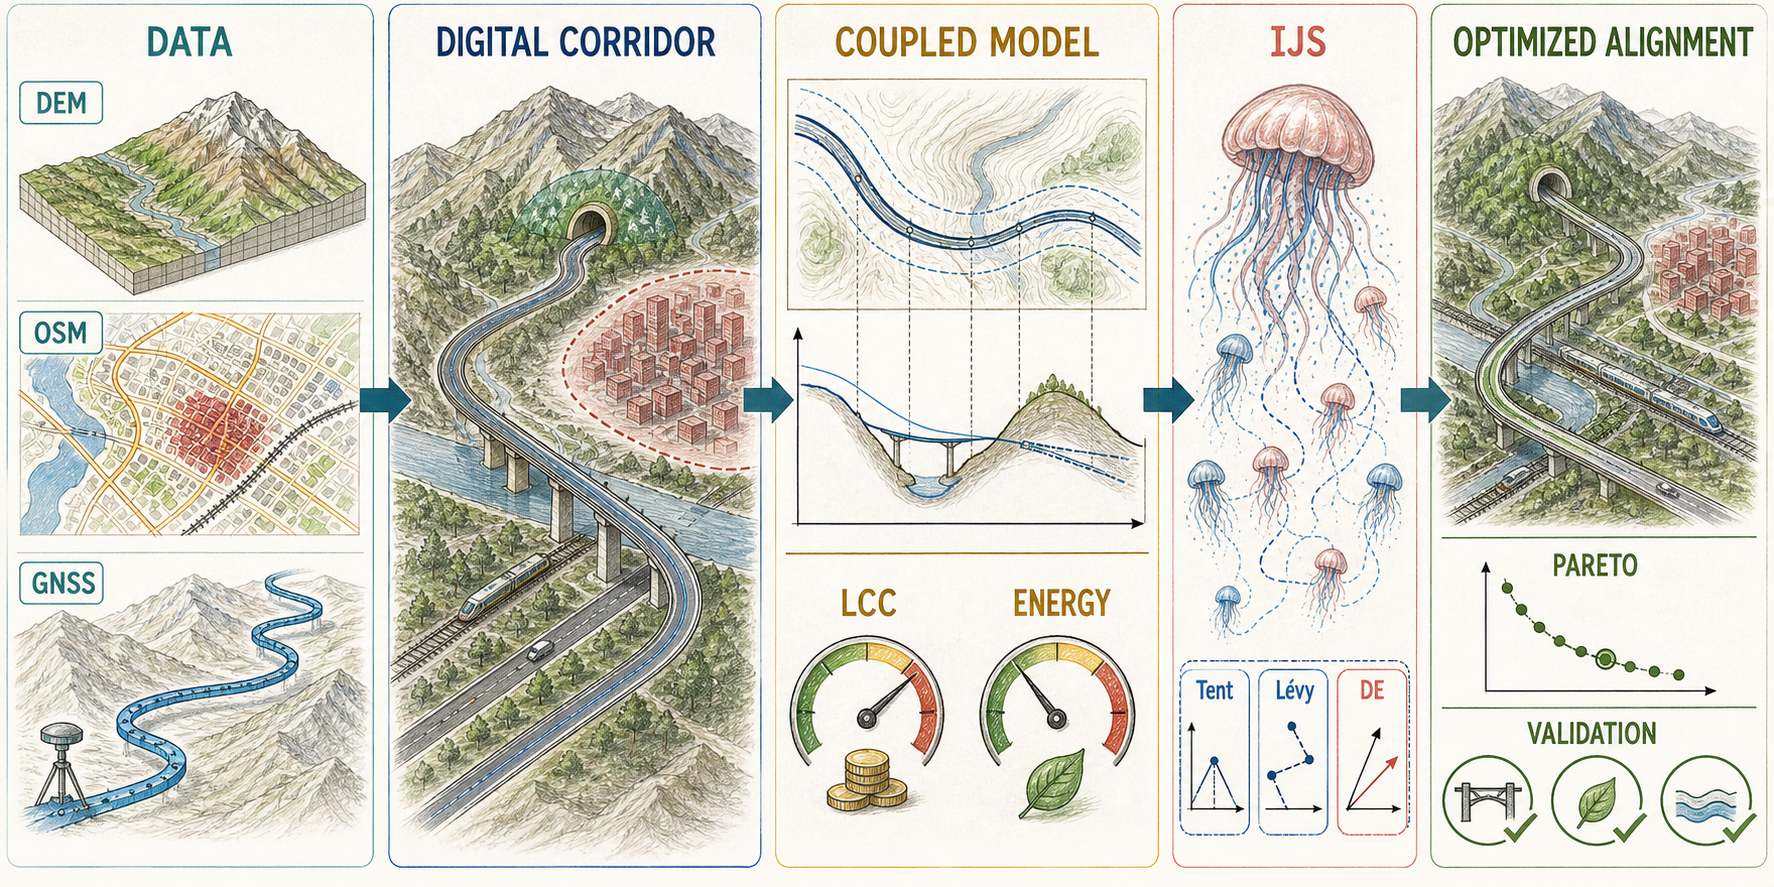
\includegraphics[width=\textwidth]{method_overview_handdrawn.png}
\caption{高速公路三维线形数据驱动协同优化方法总览。手绘科研图用于表达信息流，数学定义见第3、4节。}
\label{fig:overview_zh}
\end{figure*}

\section{相关研究}

\subsection{三维线形与空间数据}

Chew等\cite{chew1989}较早建立平纵同步优化模型，Jong和Schonfeld\cite{jong2003}进一步采用进化编码处理三维非凸搜索。此后，GIS环境约束、指定走廊平面优化和双目标三维线形得到发展\cite{kang2012,mondal2015,hirpa2016}。V\'azquez-M\'endez等\cite{vazquez2018}将基础设施成本纳入三维模型，Akhmet等\cite{akhmet2022}对公路纵断面双目标问题进行更严格求解。BIM端到端设计、低碳强化学习和3D-RRT*等新方法进一步提升了自动化程度\cite{han2023,he2023,pu2024}。这些研究表明，算法进步必须与可解释的地形—结构—规范映射同时推进。

\subsection{全生命周期成本与车流能耗}

本文沿用学位论文\cite{lin2025}的占地、桥隧、基本建设、养护和土方费用体系，并将其重新映射到候选三维线形。线形一致性会显著影响车辆排放\cite{llopis2019}；电动车能耗又受到纵坡、质量、附属能耗和再生制动的共同影响\cite{dimartino2022}。为避免直接相加升、千瓦时等不相容量纲，本文在30年分析期内将油耗和电耗货币化，但保留燃油与电动两类分项，避免把货币指标误写为唯一环境指标。

\subsection{算法与多目标决策}

NSGA-II是常用多目标基准\cite{deb2002}，但高维纵断面变量会显著增加进化搜索负担。JS模拟水母随洋流运动及主动/被动运动\cite{chou2021}。本文在JS上增加Tent、L\'evy和DE\cite{storn1997}，并通过消融判断各组件是否真正有效。熵权法以Shannon信息量为基础\cite{shannon1948}；本文先进行硬可行、预算和非支配筛选，再在剩余前沿中定权选点，从程序上禁止“权重抵消违约”。

\section{数据驱动数学模型}

\subsection{工程案例与数据融合}

案例为广州北环高速浔峰洲—黄村段，双向六车道，实测中线长22.462 km。14,018个GNSS点提供平面坐标、高程、现状方案M-A、固定平面端点和接线高程。

地形来自AWS Terrain Tiles\cite{awsterrain}的60幅z14瓦片，像元约8.8 m。由于该DEM反映现状地表，模型先掩膜实测中线两侧60 m道路影响带，再以邻域插值重建“准天然地面”，并进行1.57 m垂直基准校正；与实测中线高程的相关系数为0.915。该方法不能替代建路前测量，但保证M-A与候选方案采用同一土方口径。

OSM\cite{haklay2008,osmlicense}提供道路、铁路、水系和建筑轮廓。剔除北环自身及伴行线后，障碍物包括4,807条道路、857条铁路和338条河流/运河。建筑轮廓在25 m网格上栅格化，并以200 m尺度平滑；阈值按现状线所能穿越的最大密度标定，形成Tier 2硬禁行、Tier 1可穿越但抑制、Tier 0自由三类。图\ref{fig:case_zh}给出多源数据在局部工程坐标系中的叠加关系。

\begin{figure*}[t]
\centering
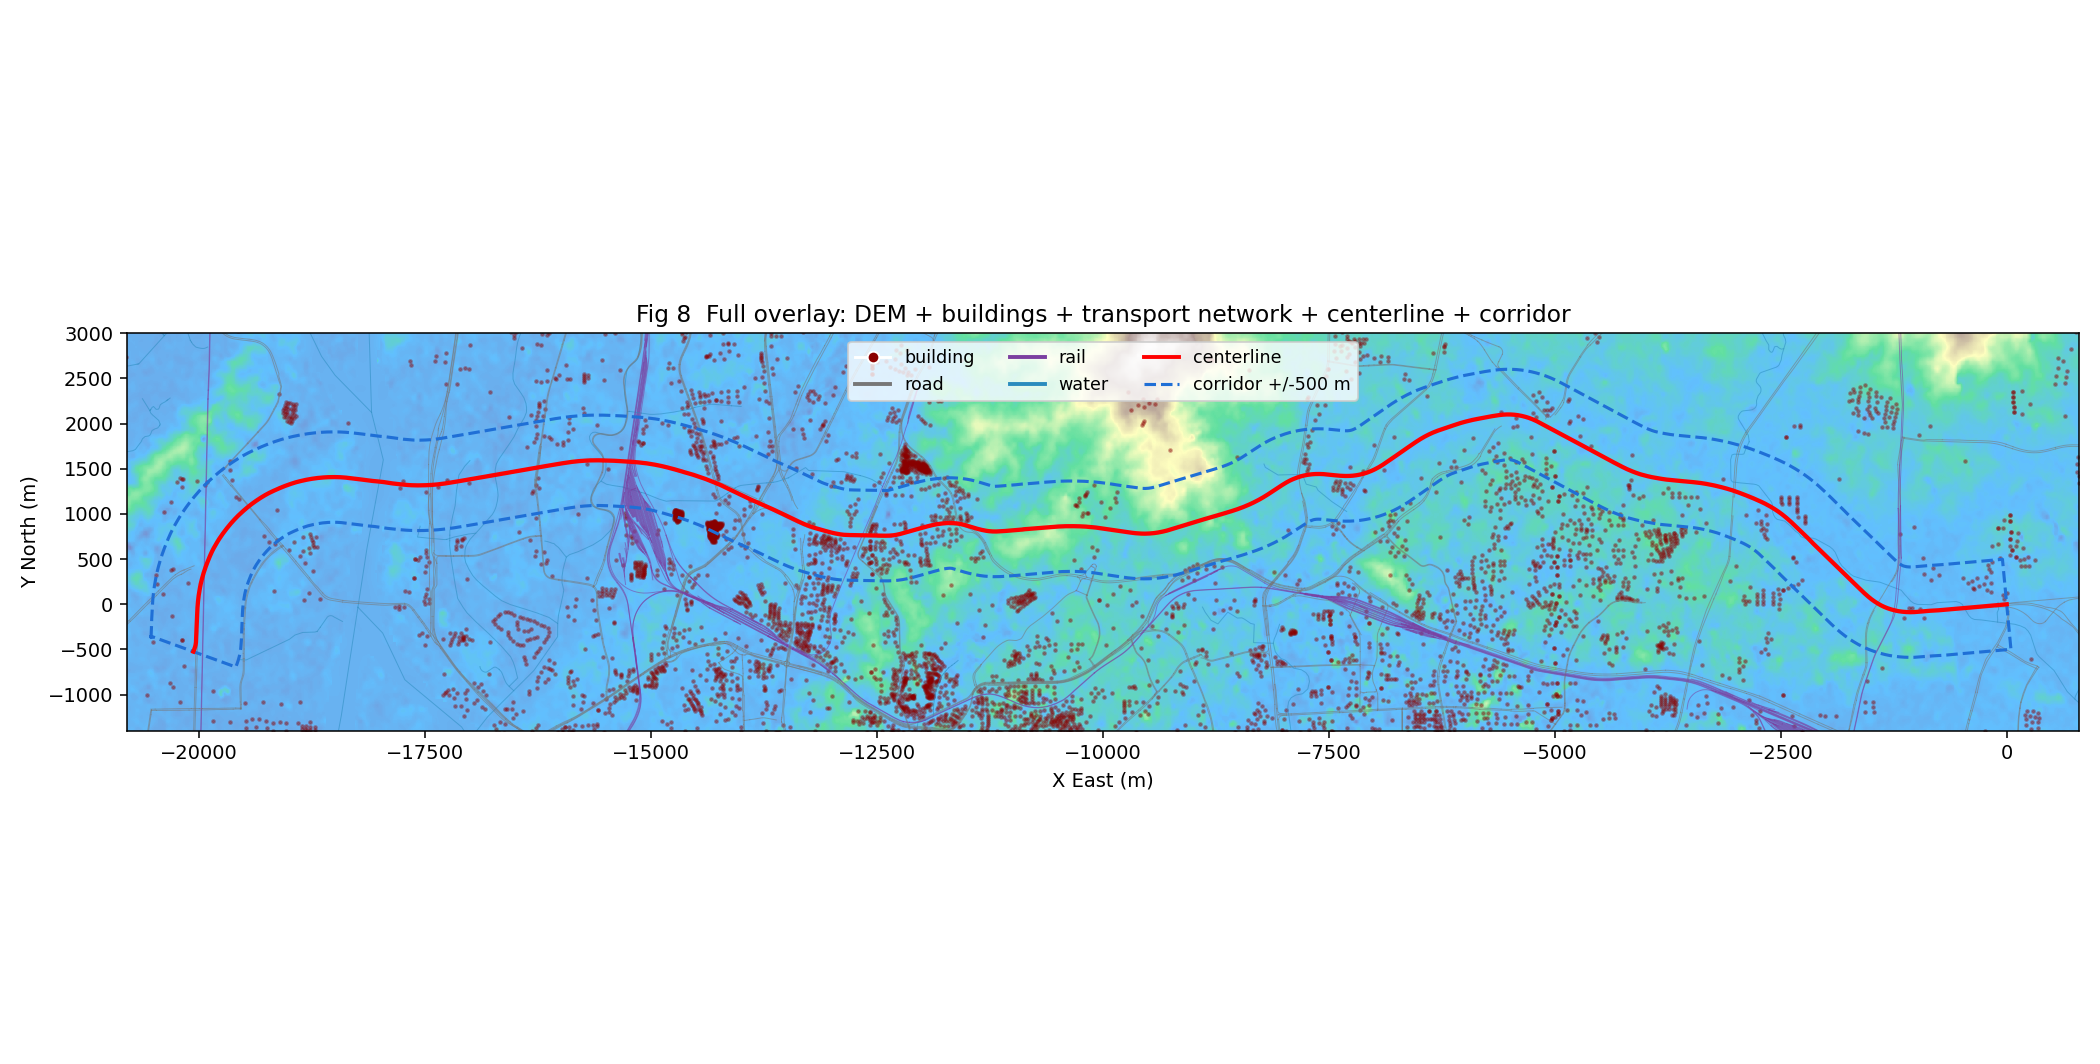
\includegraphics[width=\textwidth]{case_data_layers.png}
\caption{案例区DEM、OSM建筑/道路/铁路/水系、实测中线及$\pm500$ m走廊带叠加。}
\label{fig:case_zh}
\end{figure*}

\subsection{平纵协同决策变量}

设实测平面线为$\bm r_0(s)=[x_0(s),y_0(s)]^\top$，单位法向为$\bm n(s)$。候选平面以法向偏移表示：
\begin{equation}
\delta(s)=\sum_{k=1}^{50}a_k\sin\left(\frac{k\pi s}{L_0}\right),\qquad
|a_k|\leq \frac{W}{k^2},
\label{eq:sine_zh}
\end{equation}
主实验$W=500$ m。正弦基在两端为零，天然固定起终点；$1/k^2$衰减抑制高频曲率。控制点经三次样条重建，所有目标与约束在约10 m桩号网格上计算。

纵断面采用225个变坡控制量，间距约100 m。为固定首末接线高程，令原始坡度扰动$h_i\in[-1,1]$、坡段长$\Delta s_i$、最大纵坡$g_{\max}=0.04$，则
\begin{align}
\bar h&=\frac{\sum_i h_i\Delta s_i}{\sum_i\Delta s_i},\qquad
g_{\mathrm{req}}=\frac{z_L-z_0}{\sum_i\Delta s_i},\\
g_i&=g_{\mathrm{req}}+\lambda g_{\max}(h_i-\bar h),
\label{eq:grade_zh}
\end{align}
其中$\lambda$取保证$|g_i|\leq g_{\max}$的最大缩放值。因此$\sum_i g_i\Delta s_i=z_L-z_0$恒成立，优化器无法通过整体下倾获取虚假节能。实际优化维数为$50+225=275$，约150个平面重建控制点不属于决策维数。

\subsection{全生命周期成本目标}

成本目标为
\begin{equation}
\min C=C_R+C_B+C_S+C_Q+C_{TU},
\end{equation}
分别对应占地、桥隧、基本工程、折现养护和土方调运。单价基于学位论文及《广州市本级政府投资项目估算编制指引（2025版）》\cite{guangzhou2025}，分析期30年、折现率5\%。

设桩号$j$的设计—地面高差为$h_j=z_j-z^g_j$、路基宽度为$B$、边坡率系数为$m$，断面面积近似为
\begin{equation}
A_j=B|h_j|+mh_j^2.
\end{equation}
土方体积采用平均断面法积分。当填/挖单价超过桥/隧单价，或高填深挖超过30 m时，触发结构替代；结构区土方豁免，从而避免结构和土方重复计价，也避免“全线悬浮但免费”的退化解。

候选线形与OSM主干道路、铁路或水系相交时触发跨越桥。若障碍宽度为$b_q$、交角为$\theta_q$，桥区长度为
\begin{equation}
\ell_q=\frac{b_q}{\max(\sin\theta_q,\sin15^\circ)}+2E_{\mathrm{ext}},
\end{equation}
其中$E_{\mathrm{ext}}=75$ m，相邻间隙小于100 m则合并。七座既有立交的匝道功能费以现状校准常数计，主线桥长度则由几何内生。DEM中高程不低于70 m的连通山体经500 m闭运算形成白云山生态强制隧道区；其面积19.2 km$^2$、M-A穿越1.28 km，与独立资料约21 km$^2$、1.35 km接近。

\subsection{油电混行能耗目标}

30年货币化能耗为
\begin{equation}
\min E=\sum_{y=1}^{30}\frac{365Q_y}{(1+r)^y}
\left[(1-p_{EV})c_fe_f(\bm x)+p_{EV}c_ee_e(\bm x)\right],
\end{equation}
其中基准AADT为30,000辆/日，$p_{EV}=0.30$，油价8元/L、电价0.8元/kWh。燃油车受空气、滚动、坡度和残余横向阻力共同作用：
\begin{align}
F_{air}&=\tfrac12\rho C_dA_fv^2, & F_r&=C_rm_vg\cos\alpha,\\
F_g&=m_vg\sin\alpha, &
F_a&=\max\left(0,\frac{m_vv^2/R-m_vgS_p}{N_vC_s}\right).
\end{align}
原论文式(4.12)末尾的$10^{-3}$会使横向阻力比空气阻力低约五个数量级，使平曲线对能耗几乎无影响，故当前代码按量纲校核删除该项，并在本文显式声明。电动车采用同类受力、传动/放电效率、制动能量符号和15 kWh/100 km附属能耗。当前主实验计算代表行驶方向，端点锚定消除了净落差套利；双向平均仍作为后续完善内容。

\subsection{约束与折中决策}

硬约束包括平纵端点固定、走廊带、$R(s)\geq400$ m、$|g_i|\leq4\%$、相邻坡差、交叉角不小于$15^\circ$以及Tier 2穿越为0；规范值来自JTG D20—2017\cite{jtgd20}。局部违约采用“相对违约均值+最大值”，防止短区段严重违约被22 km线路平均掉。

同一基准种群产生$C_{ref},E_{ref}$和熵权$w_C,w_E$，标量目标为
\begin{equation}
F(\bm x)=w_C\frac{C}{C_{ref}}+w_E\frac{E}{E_{ref}}+P(\bm x)
+0.22\frac{L_{T1}}{L}.
\end{equation}
权重扫描后依次执行硬可行、预算$C\leq1.1C_{M-A}$、非支配和前沿熵权四步筛选。

\section{改进水母搜索算法}

\subsection{算法机制}

原始JS在洋流运动与种群内主动/被动运动之间切换\cite{chou2021}。本文IJS进行三项改进：
\begin{itemize}[leftmargin=*]
\item \textbf{独立Tent初始化：}每个个体使用独立混沌链且$\mu=1.99$；避免$\mu=2$在float64中塌缩为0，也避免单链造成个体相关。
\item \textbf{搜索域缩放L\'evy飞行：}步长乘$0.01(\bm u-\bm l)$；原未缩放实现的接受率仅0.48\%。
\item \textbf{DE精修：}以种群差分构造变异和交叉向量（$CR=0.5$），并采用精英接受\cite{storn1997}。
\end{itemize}

因此IJS每代约包含3倍种群评价量，本文同时报告NFE/时间，避免把同代数误认为同预算。惩罚采用前半程0.3倍、后半程3倍的两阶段调度。图\ref{fig:flow_zh}给出算法闭环。

\begin{figure}[t]
\centering
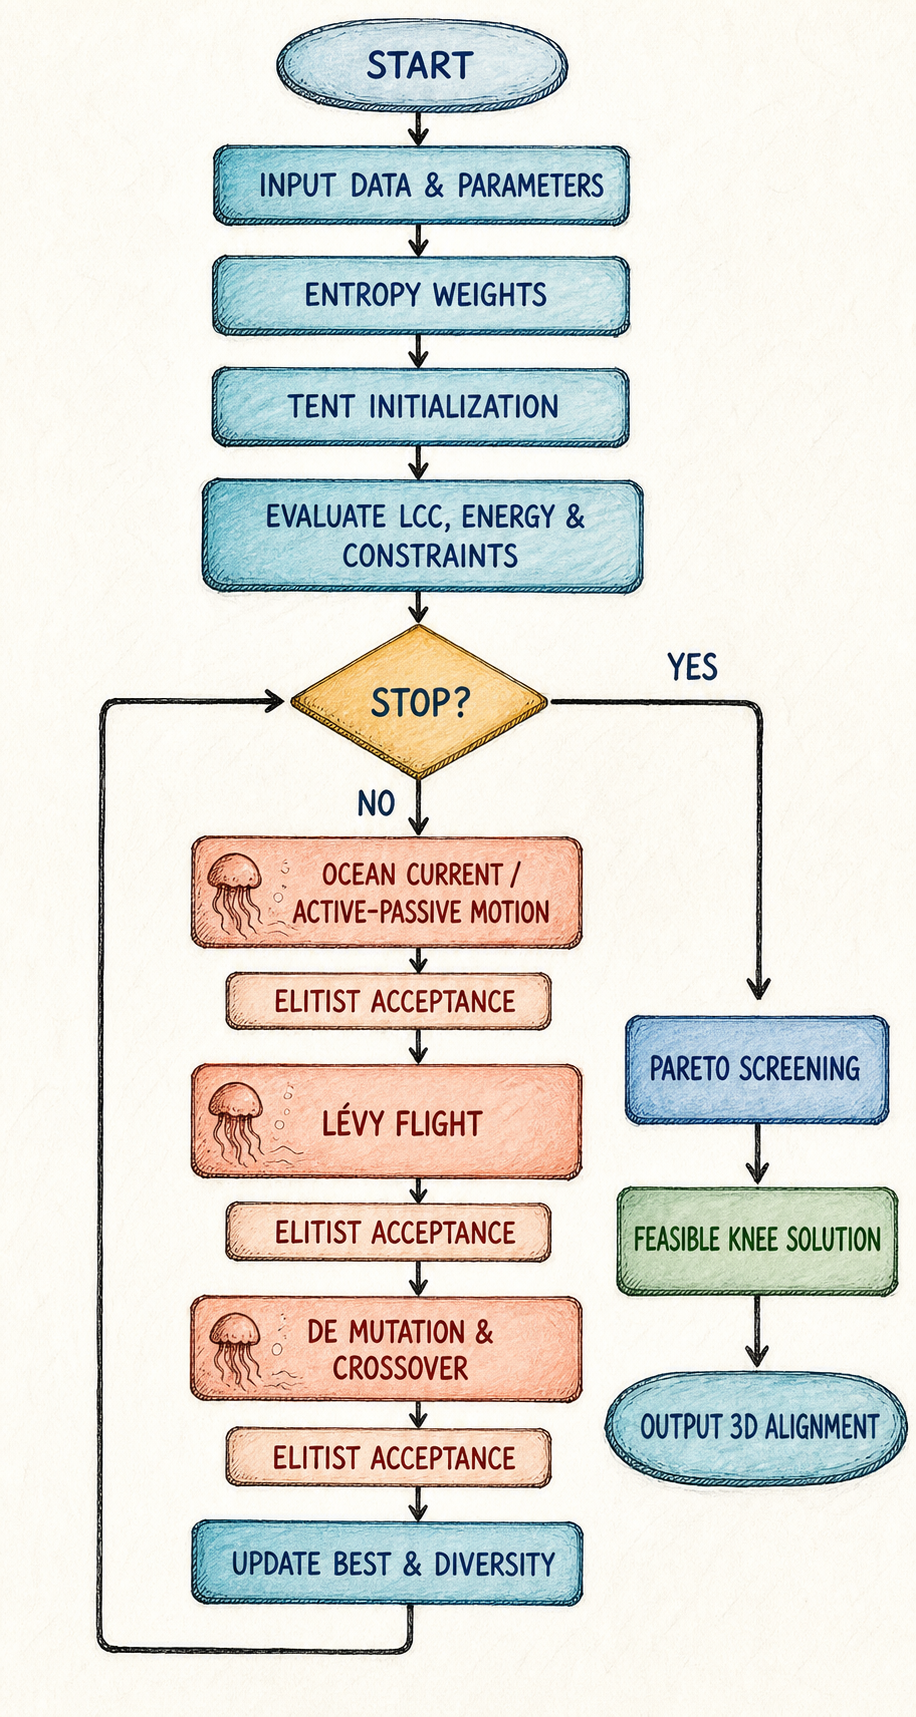
\includegraphics[height=.72\textheight,keepaspectratio]{ijs_flowchart_handdrawn.png}
\caption{IJS算法流程。每个算子之后均进行精英接受，满足停止条件后再进行Pareto筛选。}
\label{fig:flow_zh}
\end{figure}

\subsection{实验协议}

主方案采用种群200、迭代1,000、21个权重点，目标与约束在10 m网格评价。消融实验固定实测平面，求解225维纵断面，报告JS、+Tent、+L\'evy、+DE及完整IJS五个变体；每个变体30个种子、种群200、迭代500。多算法实验比较IJS、JS、NSGA-II、实数GA、PSO和GWO，纵断面步长依次为500/400/300/200/100/50 m，对应联合维数95--500，每个组合10个种子，采用Wilcoxon和Friedman检验\cite{wilcoxon1945,friedman1937}。敏感性分析在每个采样点重新优化，不以固定方案代替重优化。

\section{实验结果}

\subsection{当前工程方案}

表\ref{tab:current_zh}与图\ref{fig:scheme_zh}为当前主结果。M-C使$C$降低8.33\%、$E$降低3.00\%。线长增加12 m（+0.05\%），说明收益并非来自人为缩短线路；桥隧费减少2.37亿元，而土方费增加0.15亿元。其工程含义是：优化器接受了略长线路和更多土方，以换取更低结构暴露和运行能耗。

\begin{table}[t]
\centering
\caption{当前端点锚定、建筑密度约束开启的方案对比。}
\label{tab:current_zh}
\begin{tabular}{lrrr}
\toprule
指标 & M-A现状 & M-C优化 & 变化 \\
\midrule
全生命周期成本（亿元） & 26.4061 & 24.2078 & $-8.33\%$ \\
车流能耗（亿元） & 13.9460 & 13.5278 & $-3.00\%$ \\
里程（km） & 22.4618 & 22.4741 & $+0.05\%$ \\
最小平曲线半径（m） & 422 & 421 & 合规 \\
边坡危险度 & 3.309 & 3.298 & $-0.35\%$ \\
Tier-1穿越（km） & 约2.00 & 1.591 & $-20.5\%$ \\
Tier-2穿越（km） & 0 & 0 & 合规 \\
硬约束罚值 & 0 & 0 & 合规 \\
\bottomrule
\end{tabular}
\end{table}

\begin{figure*}[t]
\centering
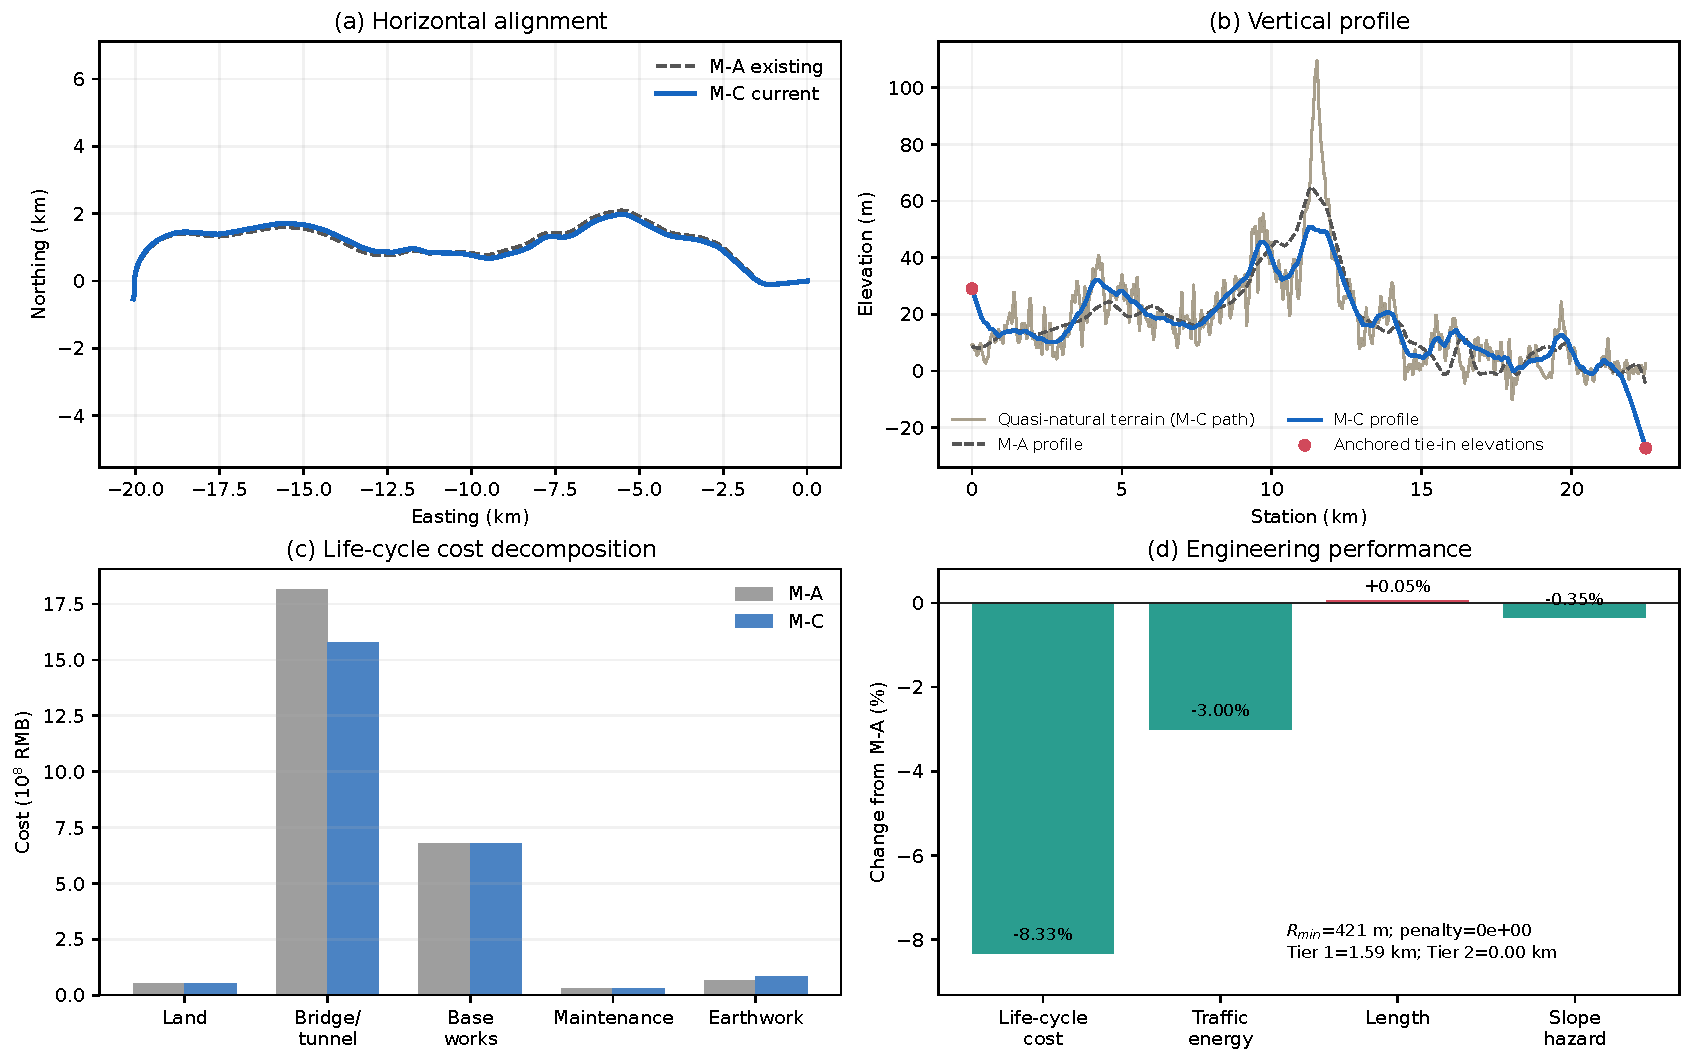
\includegraphics[width=\textwidth]{current_scheme_summary.pdf}
\caption{当前方案对比：（a）平面线形；（b）端点锚定纵断面；（c）全生命周期成本分解；（d）主要工程指标。}
\label{fig:scheme_zh}
\end{figure*}

M-C穿越Tier 1为1.591 km、Tier 2为0。图\ref{fig:density_zh}表明分区阈值并未为现状方案设置特殊豁免，而是以既有高速能够穿越的密度作为“可穿越”经验上界，超过该上界的连通核心才被禁行。

\begin{figure*}[t]
\centering
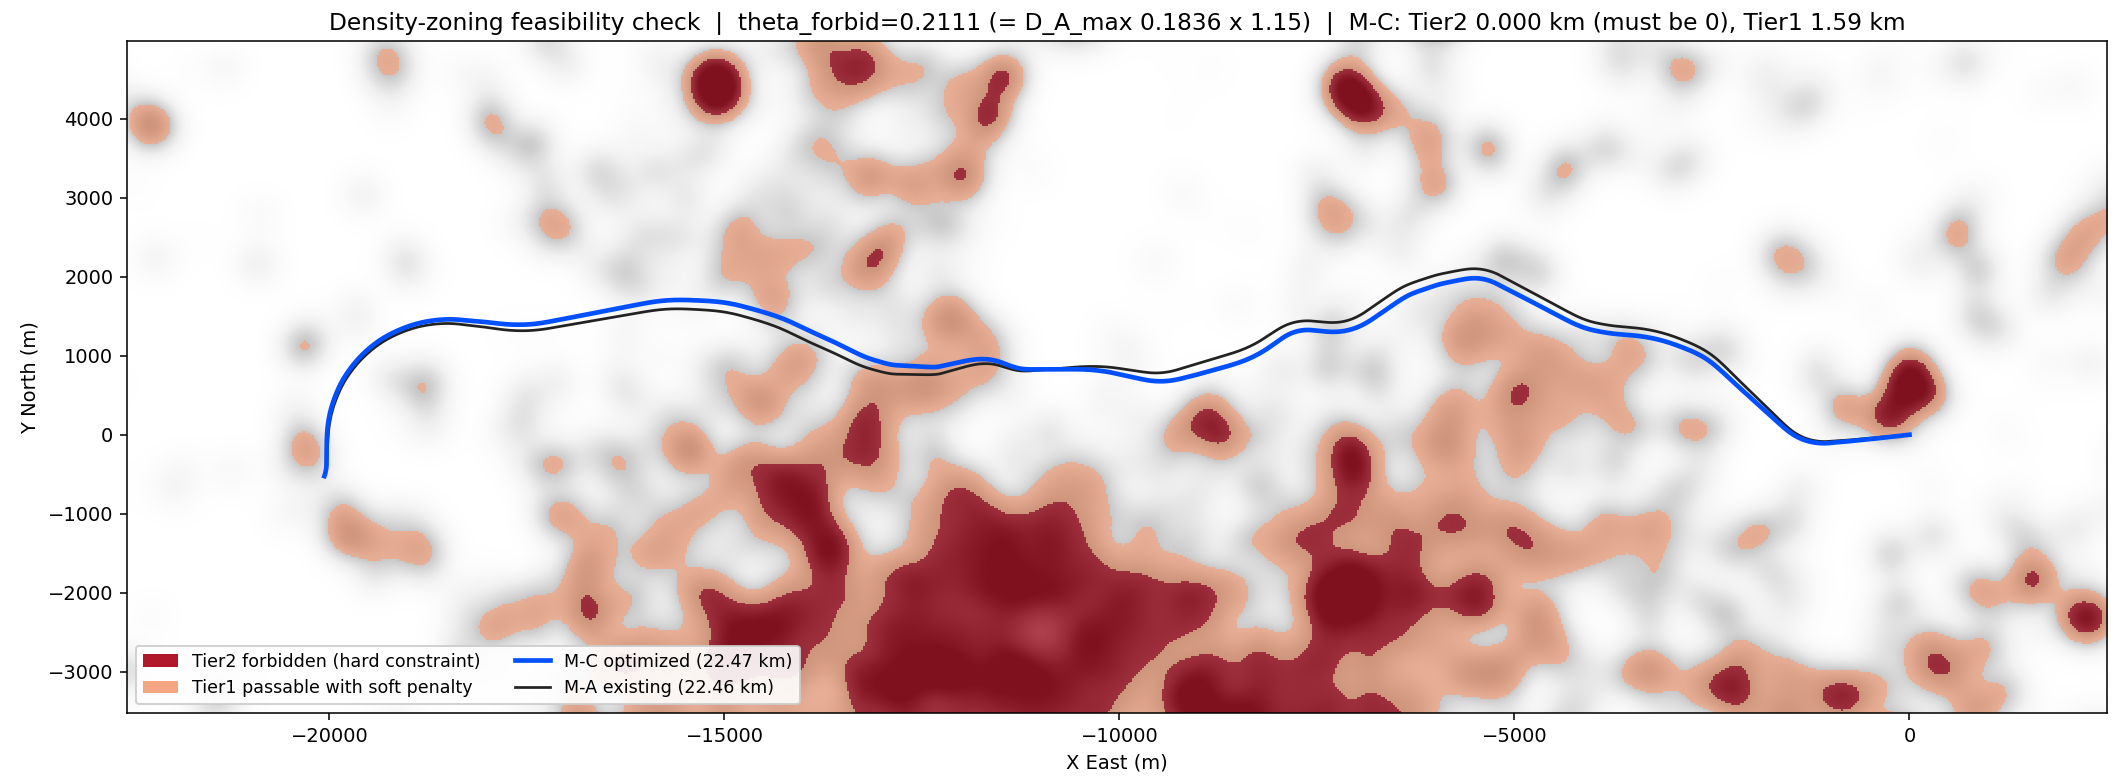
\includegraphics[width=\textwidth]{density_feasibility_w500.png}
\caption{建筑密度分区可行性核验：M-C完全绕避Tier 2，并将Tier 1穿越降至1.59 km。}
\label{fig:density_zh}
\end{figure*}

图\ref{fig:pareto_zh}的可行前沿含少量高造价、低能耗结构化端点。预算约束与非支配筛选先剔除极端方案，熵权仅在工程可接受前沿中选点，避免全局极差归一化偏向病态端点。

\begin{figure}[t]
\centering
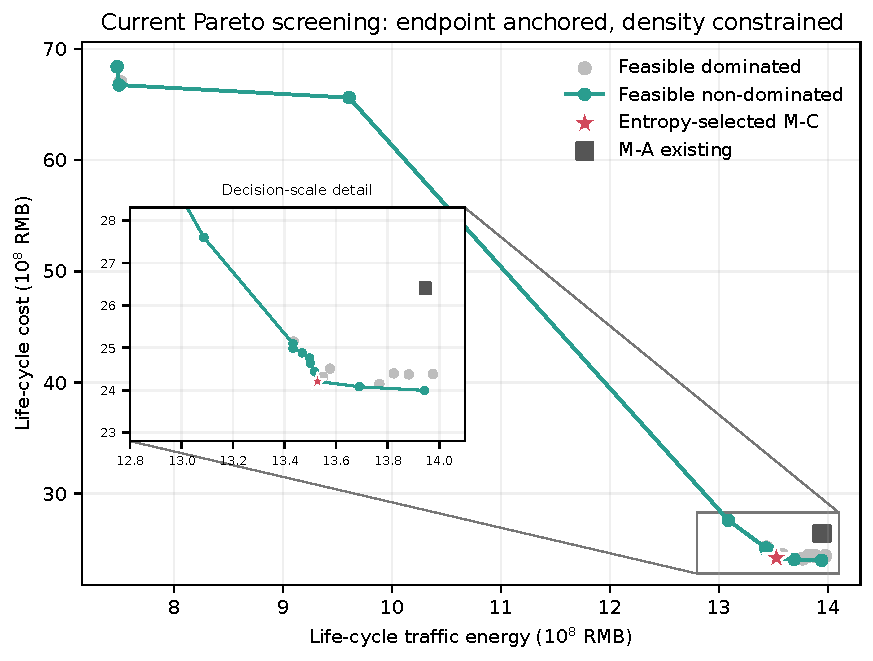
\includegraphics[width=\linewidth]{current_pareto_density.pdf}
\caption{当前端点/密度约束下的可行与非支配解筛选。}
\label{fig:pareto_zh}
\end{figure}

图\ref{fig:3d_zh}从空间上区分常规路基、OSM触发桥和生态隧道。当前M-C含约4.08 km跨越桥与0.75 km白云山生态隧道；这些数字直接来自密度约束结果，而非仓库中旧C11图的4.91/0.18 km。

\begin{figure*}[t]
\centering
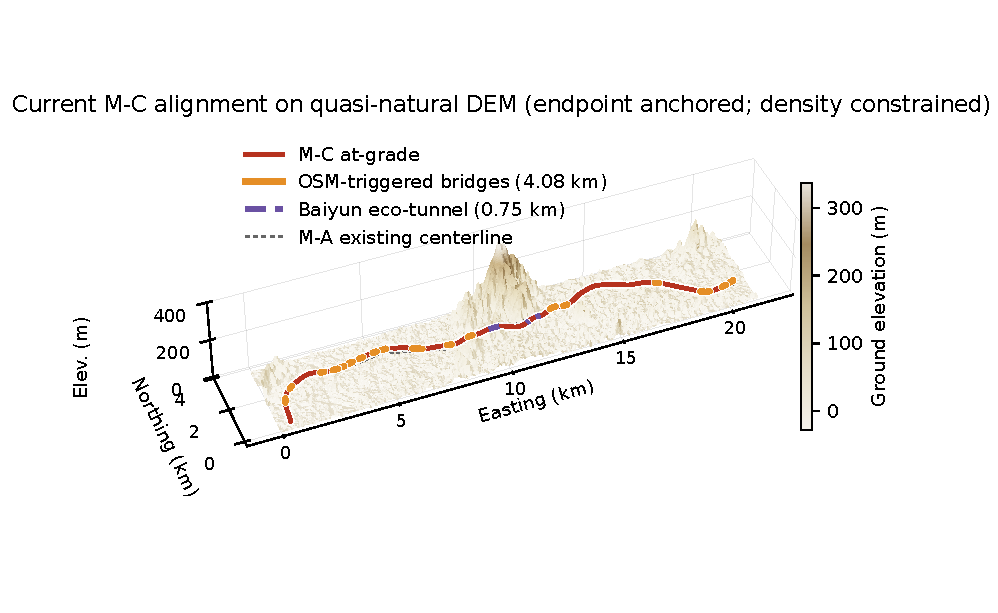
\includegraphics[width=\textwidth]{current_alignment_3d.pdf}
\caption{当前M-C在准天然DEM上的三维线形，虚线为M-A现状中线。}
\label{fig:3d_zh}
\end{figure*}

\subsection{平纵协同的必要性}

在建筑分区加入前完成的等口径、等求值预算控制实验中，两阶段方案$C=23.1582$亿元、$E=13.4569$亿元，表面优于联合方案的24.2239/13.4766亿元；但其$R_{min}=397$ m、罚值$7.36\times10^{-2}$，而联合方案$R_{min}=401$ m、罚值为0。两阶段法在第一阶段冻结平面后，纵断面已无法同时协调交叉桥位置和曲率边界。因此，本文不把不可行方案的更低目标值作为算法优势，而将其视为平纵约束耦合的直接证据。

\subsection{IJS消融实验}

表\ref{tab:ablation_zh}给出30次独立运行结果。IJS将平均$F$从0.9133降至0.6808，相对改善25.45\%；达到JS最终水平仅需187代。DE单独贡献24.17\%且显著；L\'evy改善3.79\%（$p=0.0555$）；Tent改善1.58\%但单独不显著。因此更准确的机理表述是“DE主导、L\'evy辅助、Tent改善初始覆盖”，而不是笼统宣称混沌初始化决定性能。

\begin{table}[t]
\centering
\caption{225维纵断面问题的30次IJS消融结果。}
\label{tab:ablation_zh}
\begin{tabular}{lrrrrr}
\toprule
变体 & 平均$F$ & 标准差 & $F_{100}$ & 较JS改善 & $p$ \\
\midrule
JS & 0.9133 & 0.0637 & 2.547 & -- & -- \\
JS+Tent & 0.8989 & 0.0605 & 2.227 & 1.58\% & 0.464 \\
JS+L\'evy & 0.8787 & 0.0558 & 2.095 & 3.79\% & 0.0555 \\
JS+DE & 0.6926 & 0.0315 & 1.679 & 24.17\% & $3.02\times10^{-11}$ \\
IJS & \textbf{0.6808} & 0.0340 & \textbf{1.292} & \textbf{25.45\%} & $3.02\times10^{-11}$ \\
\bottomrule
\end{tabular}
\end{table}

\begin{figure*}[t]
\centering
\begin{subfigure}{.48\textwidth}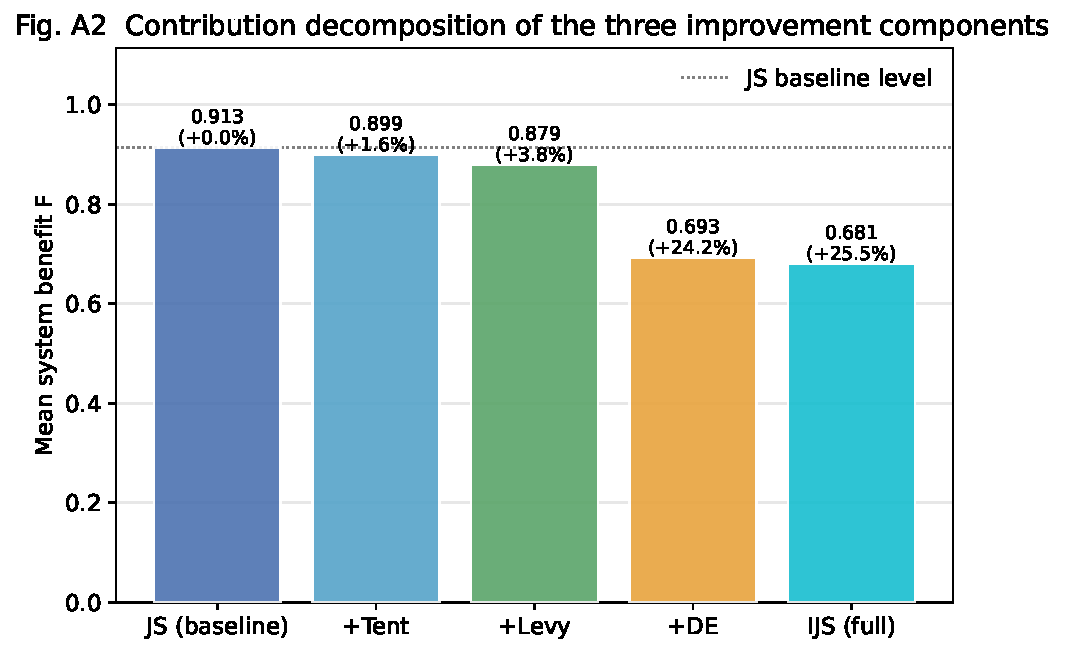
\includegraphics[width=\linewidth]{ablation_contributions.pdf}\caption{组件贡献。}\end{subfigure}\hfill
\begin{subfigure}{.48\textwidth}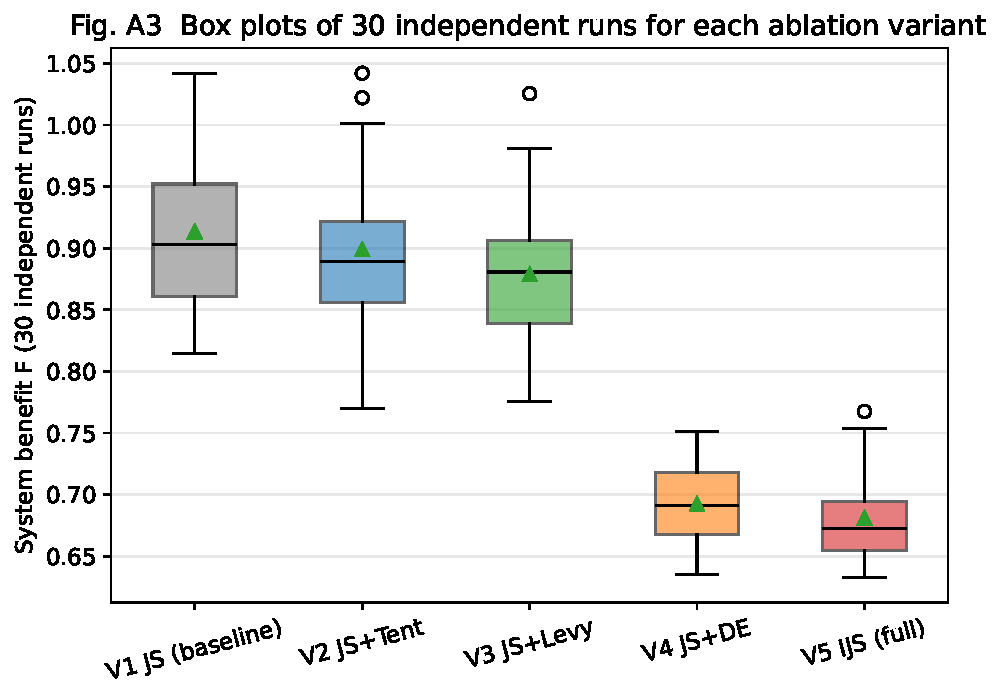
\includegraphics[width=\linewidth]{ablation_boxplot.pdf}\caption{运行分布。}\end{subfigure}
\caption{IJS消融结果，$F$越低越优。}
\end{figure*}

机制插桩显示，独立Tent链替换了200个初始个体中的132个；DE在末100代仍贡献约0.018的$F$下降，说明其不仅是早期加速，还承担后期精修。完整IJS几乎没有持续20代停滞，因此预设“停滞后逃逸率”指标不适用，不能将其机械记为0并解释为L\'evy无效。

\subsection{多算法对比}

IJS在六个联合规模上均取得最低的10次运行最优值（表\ref{tab:bench_zh}），Friedman平均秩为1.0，对各算法的Wilcoxon检验均小于$8.8\times10^{-4}$。PJ6（500维）中IJS和JS可行率为10/10，GWO为0/10，其余方法出现明显罚值主导。由于规模只改变纵断面分辨率而保持工程模型不变，该结果反映的是约束高维问题求解能力。

\begin{table*}[t]
\centering
\caption{六规模十次运行的最优$F$（越低越优）。}
\label{tab:bench_zh}
\begin{tabular}{lrrrrrr}
\toprule
算法 & PJ1（95） & PJ2 & PJ3 & PJ4 & PJ5 & PJ6（500） \\
\midrule
IJS & \textbf{0.6570} & \textbf{0.5928} & \textbf{0.7054} & \textbf{0.7053} & \textbf{0.7682} & \textbf{0.8305} \\
JS & 0.6697 & 0.5977 & 0.7127 & 0.7108 & 0.7911 & 0.8465 \\
NSGA-II & 0.6737 & 0.6095 & 0.7203 & 0.7161 & 0.7939 & 12.0355 \\
GA & 0.6939 & 0.6269 & 0.7322 & 0.7370 & 4.5169 & 23.4880 \\
PSO & 0.6841 & 0.6184 & 0.7324 & 0.7527 & 7.7130 & 31.8988 \\
GWO & 0.6715 & 0.6111 & 0.7161 & 0.7149 & 1.0843 & 1.3556 \\
\bottomrule
\end{tabular}
\end{table*}

\begin{figure*}[t]
\centering
\begin{subfigure}{.64\textwidth}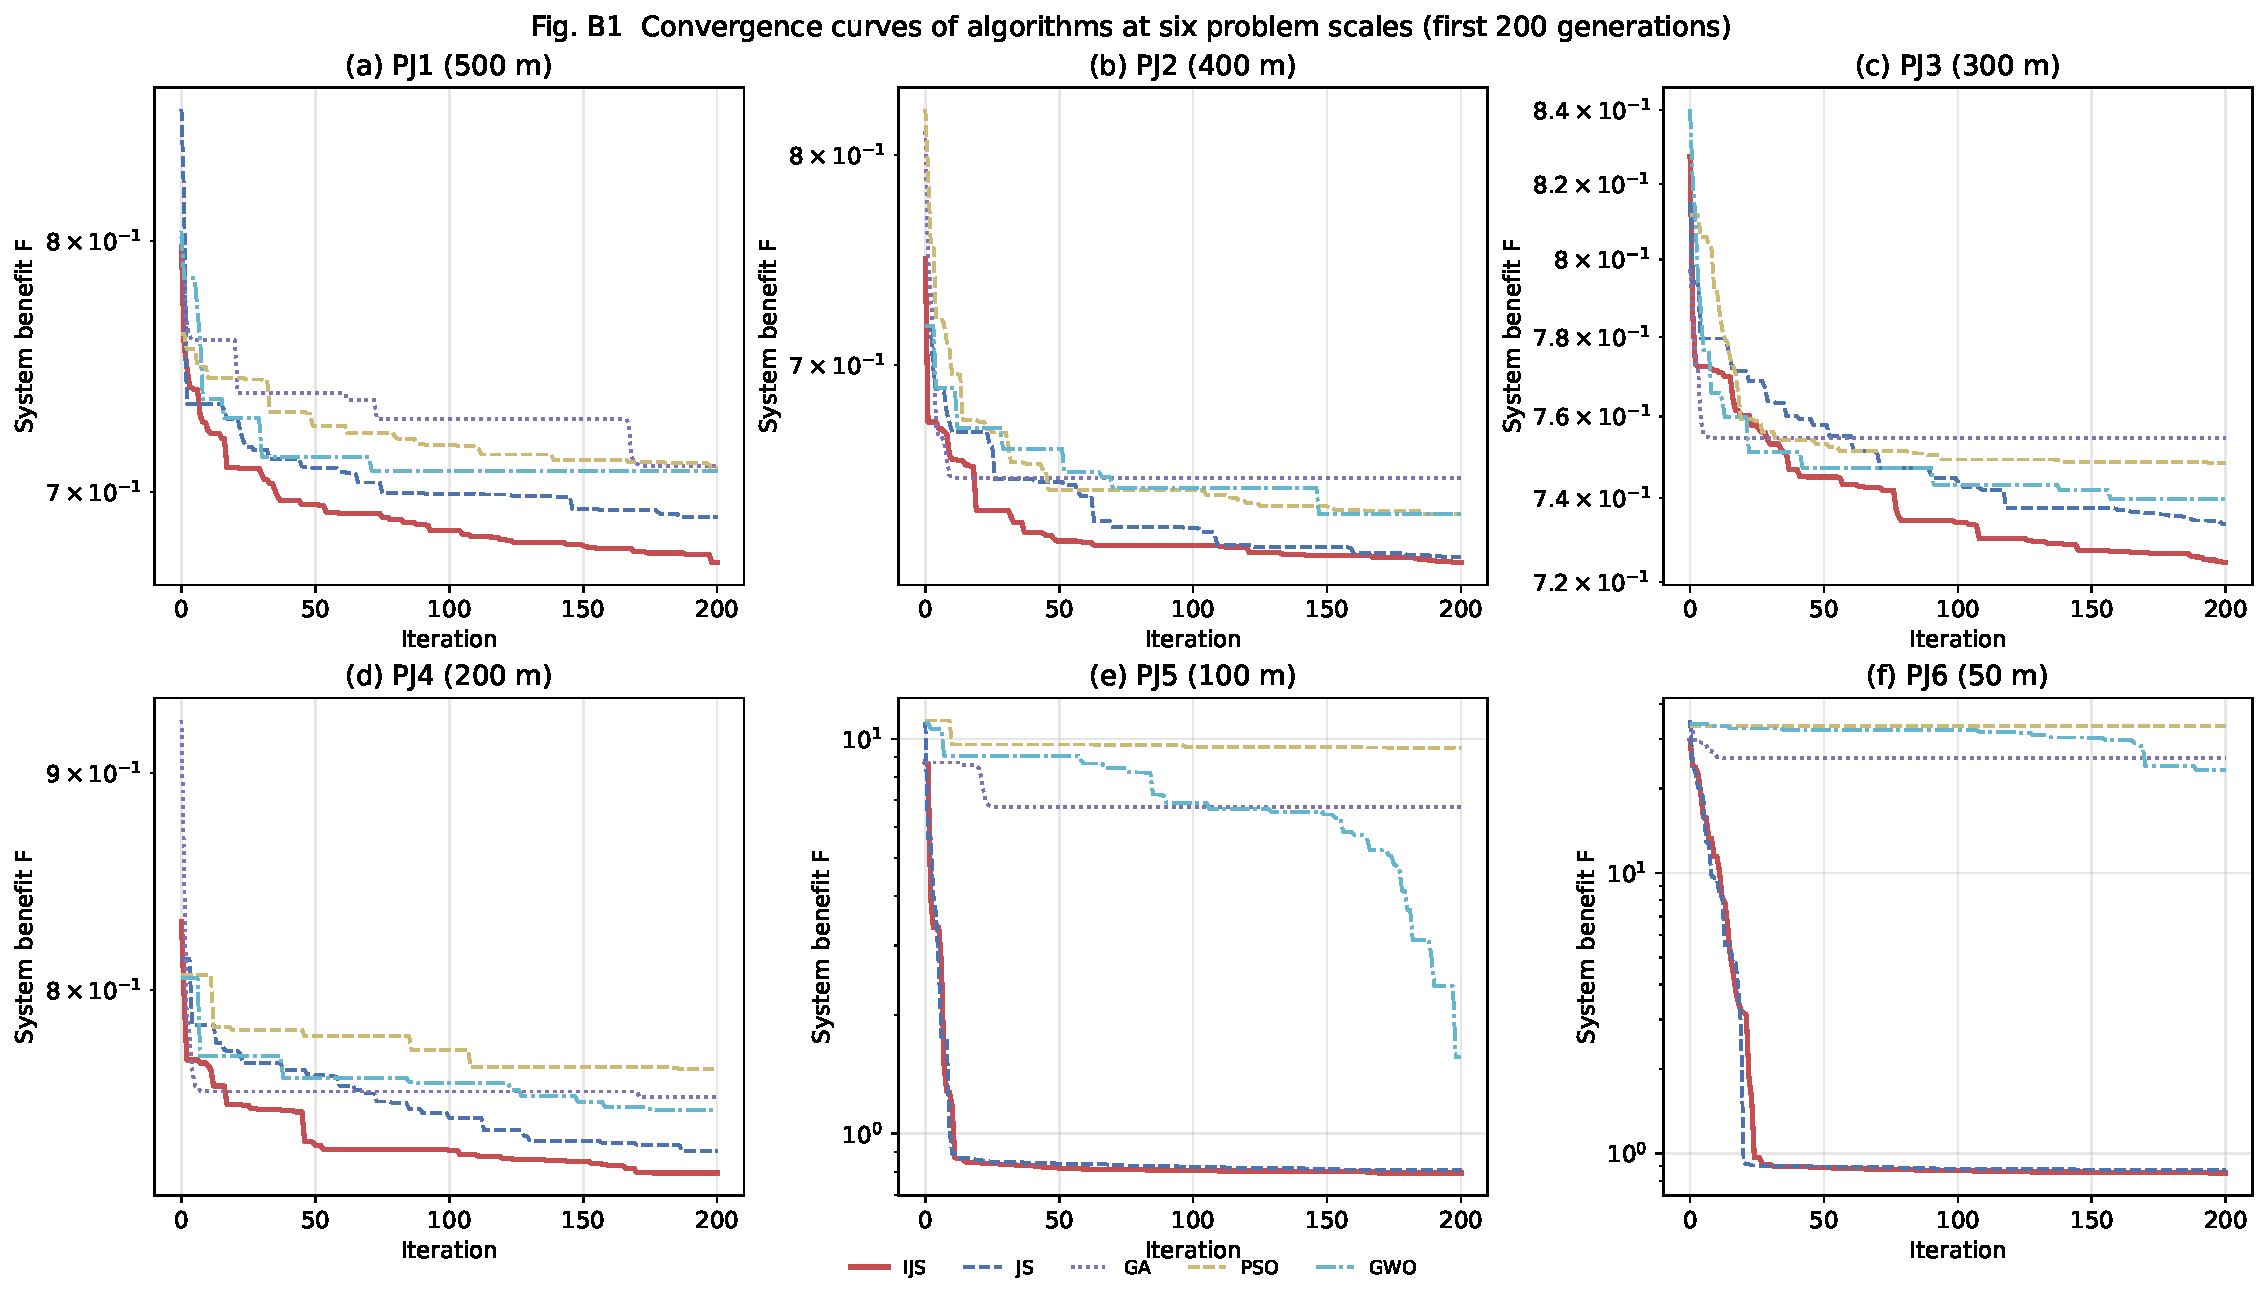
\includegraphics[width=\linewidth]{algorithm_convergence.pdf}\caption{六规模收敛。}\end{subfigure}\hfill
\begin{subfigure}{.33\textwidth}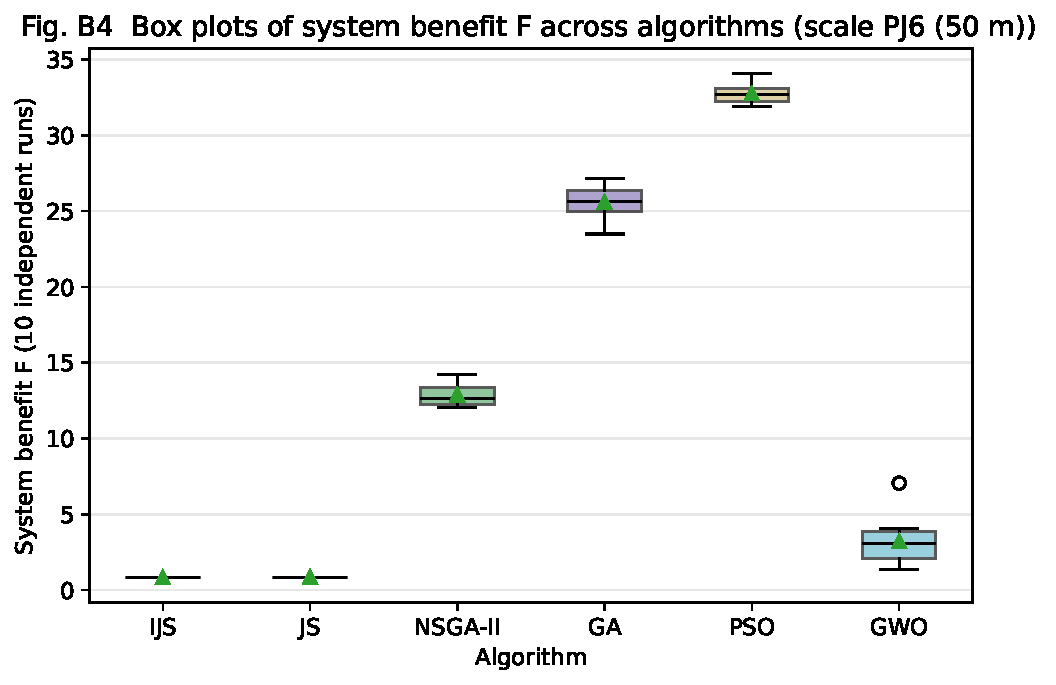
\includegraphics[width=\linewidth]{algorithm_pj6_boxplot.pdf}\caption{PJ6分布。}\end{subfigure}
\caption{多算法对比。IJS每代约3倍种群NFE，故质量、NFE和时间应同时评价。}
\end{figure*}

IJS在PJ1--PJ5的耗时约为单阶段算法的2倍，原因是L\'evy和DE增加了求值。本研究主张的是在已披露求值倍数下获得更高可行率和解质量，而非声称“相同代数下更快”。后续应进一步提供严格等NFE比较。

\subsection{重优化敏感性}

237个敏感性点全部可行。交通增长对能耗影响最大；基础设施成本在建设期发生，因而对交通、渗透率和能源价格相对稳定。提高电动车渗透率可缓解高增长情景的能耗负担，油电价格同步增长则显著抬升货币化$E$。

走廊带半宽表现出先快速、后饱和的降本规律：匹配重优化实验中，200 m时$C=25.68$亿元，2,500 m时降至22.39亿元；线位具备绕离生态隧道区的空间后，边际收益逐步受城市与曲率约束限制。桥梁两端延伸$E_{ext}=50/75/100$ m时，$C$分别为22.81/23.55/24.74亿元，而$E$保持约13.55亿元，表明该不确定工程参数主要平移结构成本，不改变能耗结论。

\begin{figure*}[t]
\centering
\begin{subfigure}{.48\textwidth}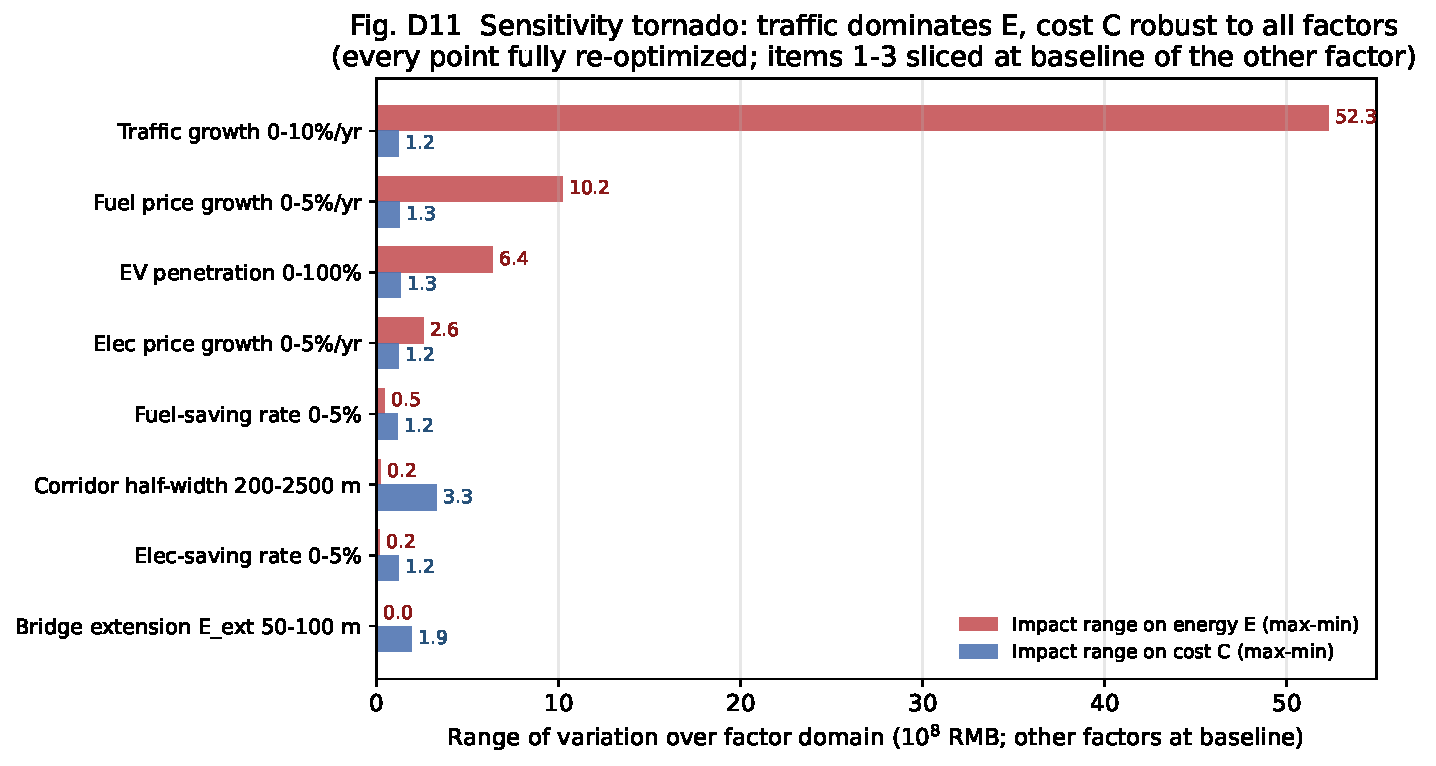
\includegraphics[width=\linewidth]{sensitivity_tornado.pdf}\caption{因素重要性。}\end{subfigure}\hfill
\begin{subfigure}{.48\textwidth}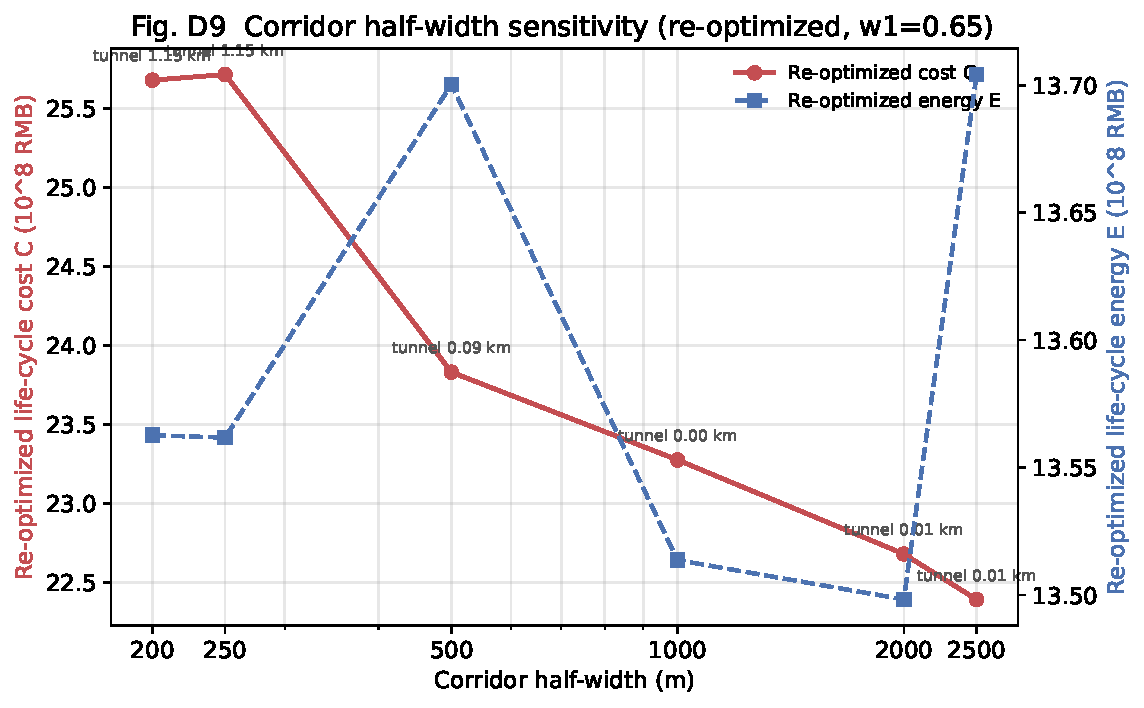
\includegraphics[width=\linewidth]{corridor_sensitivity.pdf}\caption{走廊带重优化。}\end{subfigure}
\caption{敏感性结果。每个采样点均重新优化。}
\end{figure*}

\section{讨论}

\subsection{降本节能的工程解释}

8.33\%是本案例、共同单价和共同数据下的相对变化，不能外推为所有高速公路的固定节省率。其可信性来自分项机制：M-C略长且土方更多，但桥隧和运行能耗下降，并完全绕开Tier 2。优化器在真实分项间进行交换，而不是单纯靠缩短里程。端点高程锚定进一步排除了不可接线纵断面的虚假节能。

两阶段控制说明，低目标值不是充分证据。397 m半径使其不具备可比资格。联合搜索保留了移动平面交叉位置与调整纵断面的自由度，尤其适用于跨越桥与坡度过渡相互作用的路段。

\subsection{DEM/OSM与算法创新的作用}

DEM使每条候选平面线位重新采样地面；若仍按原中线比例取高程，横移只能改变里程，平纵联合的主要土方通道被结构性抹除。OSM则把跨越结构和城市暴露与几何相交联系起来。该模型仍不等同于勘察设计：它缺乏桥面高程、地块权属和完整建筑属性，但已将早期走廊优化从一维中线提升为可复核的空间筛选。

消融也不支持“混沌初始化决定一切”的叙事。Tent单独效应小且不显著，DE解释绝大多数改善，L\'evy提供中等探索。三者的互补关系与窄可行域相符：Tent改善覆盖、L\'evy提供非局部跳跃、DE精修耦合向量。高维对比中，可行率本身就是算法结果；IJS的额外求值成本只有在可行性和质量提升具有工程价值时才合理。

\subsection{局限性与效度边界}

\begin{enumerate}[leftmargin=*,label=(\arabic*)]
\item 准天然DEM由现状道路影响带重建，并非建路前实测；8.8 m像元不能表达局部排水、挡墙和微地形。
\item OSM完整性不均。secondary道路不触发桥；缺少被交设施结构高程，暂不能实施竖向净空；15°交角按现状最小15.6°校准。
\item Tier-1权重0.22属于规划抑制项，不是实测拆迁费用。最新密度约束仅用于当前方案实验；消融与算法对比采用共同的密度加入前目标，故属于算法证据而非当前方案的直接重复。
\item 能耗目标为货币量且只计算代表方向。端点锚定解决净落差套利，但最终设计需要双向交通加权和经标定的再生制动。
\item 相邻坡差只是竖曲线代理；尚未显式实施凸/凹竖曲线长度、不重叠、视距、缓和曲线/圆曲线分段和完整平纵组合约束。
\item 造价为前期估算口径，地质、水文、地块权属、施工组织、隐含碳和概率不确定性尚未进入模型。
\item 当前密度约束主方案为一次优化结果。专门算法实验具有多种子统计，但投稿前仍需对最新主方案补充多种子复现。
\end{enumerate}

因此本文结论适用于可复现的走廊级决策与方法比较，不能直接替代详细路线和施工图设计。

\section{结论}

本文提出将三维几何、全生命周期成本和油电混行能耗联系起来的高速公路平纵协同优化方法。在既有数学模型基础上，进一步引入准天然DEM、OSM交叉桥、生态隧道、建筑密度分区、结构替代和接线端点锚定，并以IJS和“先可行、再非支配、后熵权”流程求解。

广州北环高速当前$\pm500$ m密度约束方案实现成本降低8.33\%、货币化能耗降低3.00\%，最小半径421 m、硬罚为0、Tier 2穿越为0。线位略长且土方增加，说明净收益来自可解释的结构与运行权衡。两阶段控制证明，不可行的更低目标不能替代协同可行解；消融和六规模对比表明DE是IJS提升主体、IJS总体最优；237点重优化支持结论方向的稳健性。

后续应优先补充双向能耗、测量级障碍物高程、显式竖曲线与视距、地块/隐含碳目标、造价不确定性，以及最新密度方案的多种子统计，从走廊级智能比选进一步迈向设计级决策支持。

\section*{数据与代码可用性}
论文由RoadPlan实验仓库生成。GNSS及项目派生文件可能受数据所有者限制；处理后的DEM/OSM、源代码、固定随机种子、结果JSON和制图脚本已按复现逻辑组织。双盲审稿后应补充公开仓库与DOI（当前为数据仓库DOI占位符）。

\section*{作者贡献}
\textbf{[作者姓名占位]}：概念设计、方法、软件、验证、调查、数据整理、可视化、初稿、审阅与修改。投稿前须按真实分工替换。

\section*{利益冲突声明}
作者声明不存在可能影响本文工作的已知经济利益或个人关系；投稿前须由全部作者确认。

\section*{致谢}
基金名称、编号及非作者贡献因双盲审稿暂作匿名占位，投稿前补全。

\bibliographystyle{elsarticle-num}
\bibliography{../references}

\end{document}
